\documentclass[12pt,letterpaper,fleqn]{article}
\usepackage{fullpage}
\usepackage[top=2cm, bottom=4.5cm, left=2.5cm, right=2.5cm]{geometry}
\usepackage{amsmath,amsthm,amsfonts,amssymb,amscd}
\usepackage[utf8]{inputenc}
\usepackage{lastpage}
\usepackage{enumerate}
\usepackage{fancyhdr}
\usepackage{mathrsfs}
\usepackage{xcolor}
\usepackage{graphicx}
\usepackage{listings}
\usepackage{hyperref}
\usepackage{amsmath}
\usepackage{nccmath}
\usepackage{physics}

\newcommand{\R}{\mathbb{R}}
\newcommand{\Q}{\mathbb{Q}}

\newcommand{\cent}{$^{\circ}$}
\newcommand{\delfrac}[2][y]{\frac{\partial #1}{\partial #2}}


\hypersetup{%
 colorlinks=true,
  linkcolor=blue,
  linkbordercolor={0 0 1}
}
 
\renewcommand\lstlistingname{Algorithm}
\renewcommand\lstlistlistingname{Algorithms}
\def\lstlistingautorefname{Alg.}

\lstdefinestyle{Python}{
    language        = Python,
    frame           = lines, 
    basicstyle      = \footnotesize,
    keywordstyle    = \color{blue},
    stringstyle     = \color{green},
    commentstyle    = \color{red}\ttfamily
}

\setlength{\parindent}{0.3in}
\setlength{\parskip}{0.05in}

% Edit these as appropriate
\newcommand\course{Física - Frente 2}
\newcommand\hwnumber{1}                  % <-- homework number
\newcommand\NetIDa{netid19823}           % <-- NetID of person #1
\newcommand\NetIDb{netid12038}           % <-- NetID of person #2 (Comment this line out for problem sets)

\pagestyle{fancyplain}
\headheight 35pt
%\lhead{\NetIDa}
%\lhead{\NetIDa\\\NetIDb}                 % <-- Comment this line out for problem sets (make sure you are person #1)
\chead{\textbf{\Large Leis da Termodinâmica  }}
\rhead{\course \\ Outubro/2019}
\lfoot{}
\cfoot{}
\rfoot{\small\thepage}
\headsep 1.5em

\begin{document}
\begin{enumerate}
    \item Durante o \textit{reality show} Pesadelo na Cozinha, o chef de cozinha Érick Jacquin ajuda o restaurante Pé de Fava. Enquanto conhecia o restaurante, Jacquin descobre que os freezers cheio de comidas congeladas eram desligados a noite por durante 12 horas, como uma forma de economia de energia.
    
    O dono argumenta que isso não faz com que a carne descongele, porém Jacquin sabendo dos conhecimentos de Termodinâmica, diz que os alimentos estariam descongelados após 12h, mesmo que eles estejam dentro do freezer.
    
    Sabendo que o freezer, no momento que é desligado, está na temperatura de $-20^{\circ}C$, que a capacidade térmica da carne congelada é de $C_{cong}=2.5*10^2 J$, o calor latente da carne congelada é de $Q_L = 7*10^3 J$ e o capacidade térmica da carne descongelada é de $C_{desc}=2*10^2 J$. Supondo que o fluxo de dissipação de calor do freezer desligado é de $\Phi=1200 J/hora$, estime a temperatura da carne após as 12h. A carne descongelou? Jacquin tem razão para \textit{pistolar} com o dono?
    
    \item Um gás num cilindro com pistão é aquecido por microondas e exerce trabalho sobre o pistão a pressão constante, aumentando o seu volume. Sabendo que a densidade do gás é de $\rho = 3*10^{2}kg/m^3$, o volume inicial é $V_0 = 0,5 m^3$, a pressão inicial $p_0 = 3*10^2 Pa$ e o volume final $V=0.7 m^3$
    
    \begin{enumerate}
        \item Sabendo que o processo todo é isotérmico, determine o calor total do processo.
        \item Após o processo do item (a), trocamos o pistão por uma tampa fixa. Calcule o calor específico desse gás para quando injetamos a mesma quantidade de calor que obtemos no item (a), sabendo que a temperatura do gás aumentou $5^\circ C$.
    \end{enumerate}
    
    \item \textbf{(UFSM-RS)} - No gráfico estão representadas 2 isotermas e 3 transformações sucessivas $1\rightarrow 2, 2\rightarrow 3, 3\rightarrow 4$
    
    \begin{figure}[h]
        \centering
        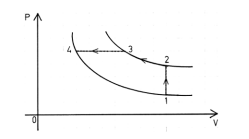
\includegraphics[width=0.6\textwidth]{ciclo.png}
    \end{figure}
    
    A sequeência de transformações são, respectivamente:
    \begin{enumerate}
        \item isométrica, adiabática, isotérmica;
        \item isotérmica, isométrica, adiabática;
        \item adiabática, isotérmica, isobárica;
        \item isométrica, isotérmica, isobárica;
        \item isobárica, isotérmica, isométrica.
    \end{enumerate}
    
    \item \textbf{(FATEC)} - Submete-se o corpo gasoso a transformações diversas:
    \begin{figure}[h]
        \centering
        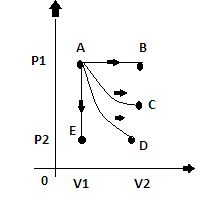
\includegraphics[width=0.4\textwidth]{fatec.png}
    \end{figure}
    
    
    \begin{enumerate}
        \item Na expansão isobárica AB, o gás cede calor (Q<0);
        \item Na expansão isotérmica AC, não intervem calor (Q=0);
        \item Na expansão adiabática AD, o gás não realiza trabalho ($\tau=0$);
        \item No esfriamento isométrico AE, o gás recebe calor (Q>0);
        \item n.d.a
    \end{enumerate}
    
    \item \textbf{(FUVEST)} - O diagrama pV da figura ilustra duas formas pelas quais o ar contido numa seringa de injeção pode ser comprimido desde um estado A até outro B. A linha curva representa uma transformação isotérmica e a reta uma transformação com temperatura variável. Admita o ar como se fosse um gás ideal.
    
    
    \begin{figure}[h]
        \centering
        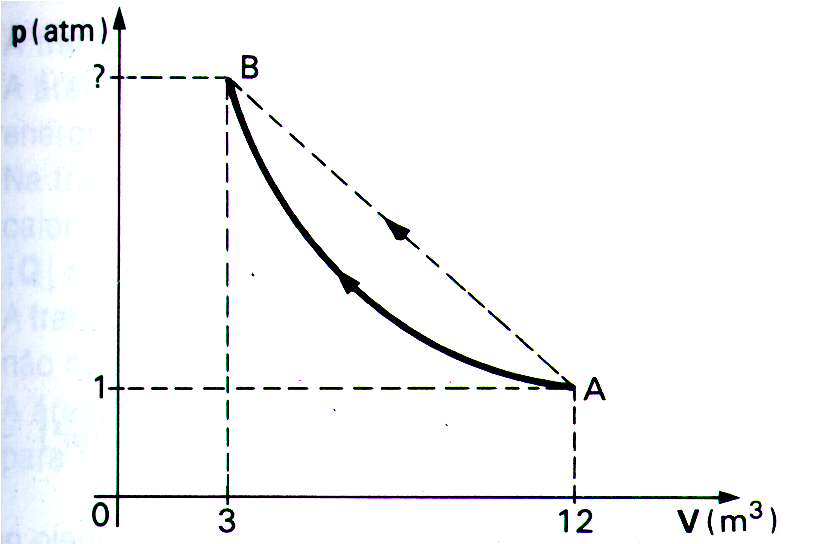
\includegraphics[width=0.5\textwidth]{fuvest.png}
    \end{figure}
    \begin{enumerate}
        \item Qual a pressão do ar no estado B? 
        \item Em qual das duas transformações o trabalho realizado é maior? Explique
    \end{enumerate}
    \pagebreak
    
    \item \textbf{(ITA - SP)} - Na expansão livre de um gás ideal, quando ele passa de um volume $V_i$ para um volume $V_f$, pode-se afirmar que essa expansão pode ser descrita por: 
    \begin{enumerate}
        \item uma expansão isotérmica;
        \item uma expansão adiabática irreversível, na qual a temperatura no estado de equilíbrio final é a mesma que no estado inicial;
        \item uma expansão isobárica;
        \item um processo isovolumétrico;
        \item nenhuma das afirmações.
    \end{enumerate}
    
    \item \textbf{(UNIOESTE)} - Um sistema termodinâmico percorre o caminho A → B → C representado no diagrama PV abaixo.
    
    \begin{figure}[h]
        \centering
        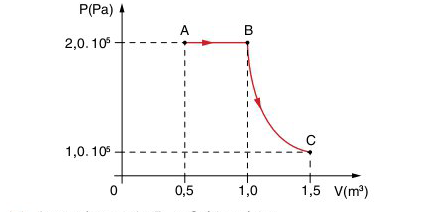
\includegraphics[width=0.5\textwidth]{unioeste.png}
    \end{figure}
Assinale a alternativa correta.

\begin{enumerate}
    \item A transformação B $\rightarrow$ C é isocórica.
    \item O trabalho realizado pelo sistema no percurso A$\rightarrow$ B é de $5,0 * 10^4 J$.
    \item Se a temperatura do sistema no ponto A for de 300 K, no ponto B será de 150 K.
    \item Se a transformação B $\rightarrow$ C for adiabática, o sistema não trocará calor com o meio externo nessa transformação.
    \item O ciclo $A \rightarrow B \rightarrow C \rightarrow A$ pode ser fechado com uma transformação isotérmica.
\end{enumerate}

\item \textbf{(UEM)} -  O diagrama abaixo representa o ciclo de Carnot realizado por um gás ideal que sofre transformações em uma máquina térmica. 
\begin{figure}[h]
    \centering
    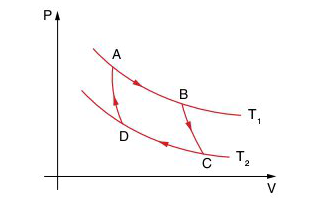
\includegraphics[width=0.5\textwidth]{uem.png}
\end{figure}

Com relação ao ciclo de Carnot, é correto afirmar que:

\begin{enumerate}
    \item o gás sofre duas expansões isotérmicas;
    \item o rendimento da máquina é de 100\%;
    \item o gás sofre uma expansão adiabática de B para C. 
    \item  o gás sofre uma compressão adiabática de C para D.  
    \item o gás sofre uma compressão isotérmica de D para
A.  
\end{enumerate}
\end{enumerate}

\pagebreak
\section*{GABARITO}
\begin{enumerate}
    \item $T=12^\circ C$
    \item
    \begin{enumerate}
        \item$Q=60 J$
        \item $c = 2 J/(Kg ^\circ C)$
    \end{enumerate}
    \item (d)
    \item (e)
    \item \begin{enumerate}
        \item $P=4 atm$ 
        \item O trabalho da linha reta é maior do que a da linha curva pois a área embaixo do gráfico é maior
    \end{enumerate}
    \item (b)
    \item (d)
    \item (c)
\end{enumerate}
\end{document}
